\section{Conteúdo dos slides}

Um slide típico, no caso geral, tem duas funções básicas, uma ligada ao momento em que ele é usado e outra ligada ao seu uso futuro.

No momento em que é usado, o slide deve servir de referência para o assunto e também para indicar o momento da apresentação, posicionando a audiência. Assim, o número do slide serve para mostrar quanto o apresentador está avançado, o título indica o assunto sendo tratado e os itens textuais e imagens mostram o detalhamento do assunto.

Para indicar melhor o momento do slide no total da apresentação, o \texttt{beamer} possui alguns temas que geram automaticamente, em cada slide, um índice que mostra o posicionamento do slide na aula. Isso é demonstrado na Figura \ref{fig:sistemas}. No cabeçalho do slide podemos ver o nome da seção e da subseção, que no caso é o mesmo nome do slide\footnote{Essa apresentação, sobre o uso do \LaTeX, está disponível em \url{https://github.com/xexeo/Seminario-LaTeX-2020}}.

\begin{figure}[tbh]
    \centering
    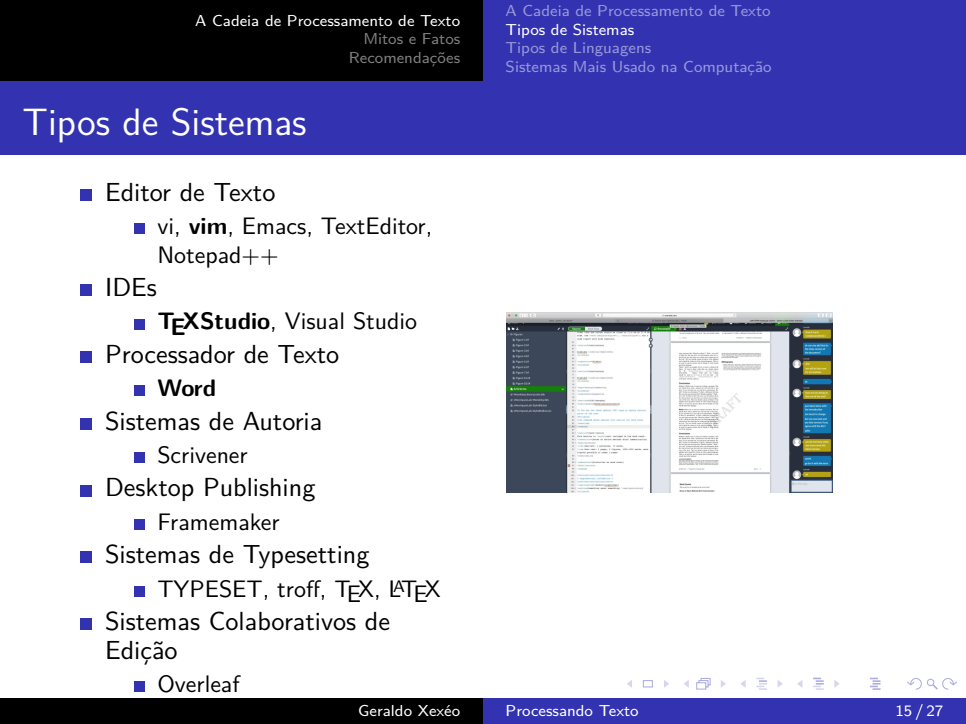
\includegraphics[width=\tam\linewidth,frame]{imagens/sistemas}
    \caption{Slide feito no \texttt{beamer} onde um índice é gerado automaticamente no topo de cada slide com o tema Luebeck}
    \label{fig:sistemas}
\end{figure}

Então, no primeiro uso, é importante trabalhar o que está sendo apresentado naquele momento, que indica um intervalo de tempo onde o slide será apresentado, dentro de toda apresentação. Dependendo do tipo de apresentação, isto pode ser feito de várias formas. Por exemplo, uma apresentação mais motivacional pode colocar apenas perguntas nos slides, e o apresentador pode respondê-las enquanto fala. Já uma apresentação formal de tese exige que o conteúdo esteja lá para referência da banca.

Já para o segundo uso, como uma leitura posterior, temos que trabalhar a qualidade da informação sendo passada. Algumas apresentações não são feitas com essa intenção, como é o caso de algumas apresentações motivacionais, mas no mundo acadêmico é uma norma geral que os slides possam ser usados como uma referência futura ao tópico, pelo menos de forma inicial.

O conteúdo típico de um slide é um lista de itens  que representa o que vai ser falado naquele momento. A menos de definições formais e informações específicas, como tabelas de dados, o conteúdo não deve ser lido de forma explícita, mas sim ser uma forma reduzida do que é falado.  Essa lista pode conter exemplos, definições, motivação, dependendo da necessidade do slide.

Por exemplo, o parágrafo anterior poderia ser dito, de forma semelhante, em um slide com o título ``Conteúdo Básico de Um Slide'':
\begin{itemize}
    \item lista de itens tratados;
    \item definições formais;
    \item tabelas e gráficos, e
    \item resumo do conteúdo da fala.
\end{itemize}

O slide da Figura \ref{fig:coppe} é um slide típico criado no \textit{Power Point}. Ele contém um título, que no caso se refere a uma categoria introduzida no slide anterior, e quatro subcategorias, que são explicadas em letras menores.

\begin{figure}[htb]
    \centering
    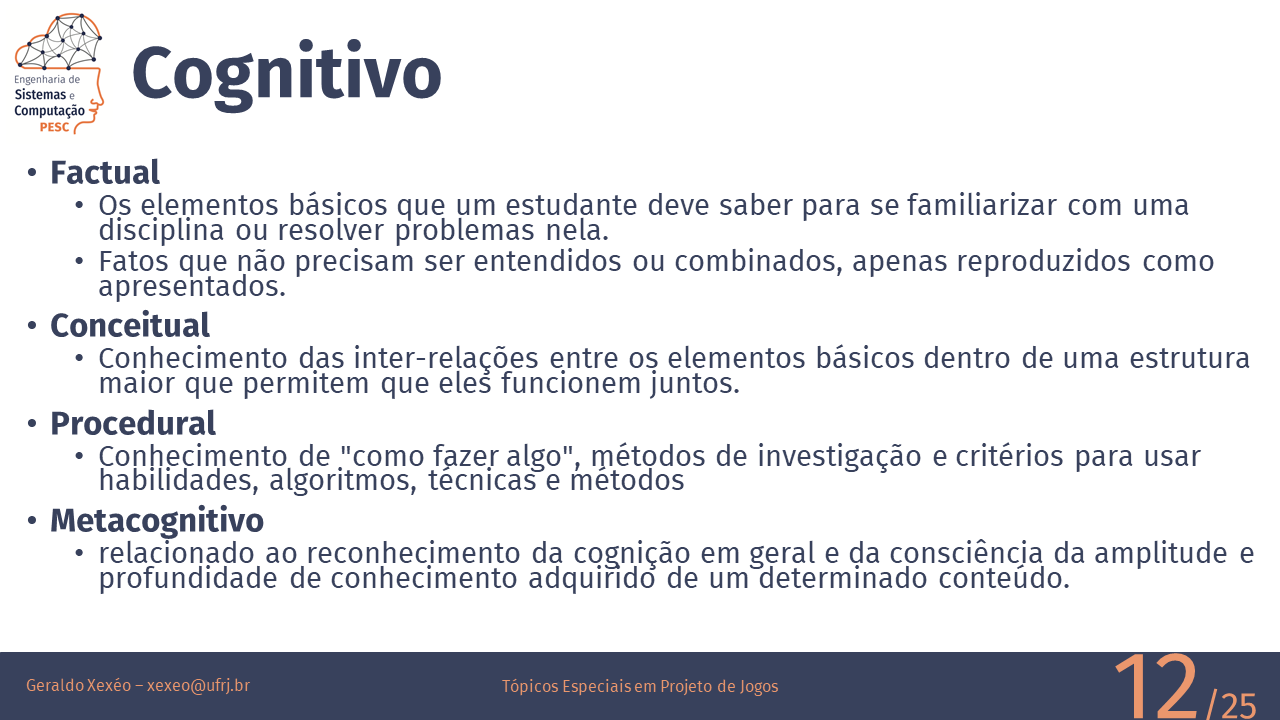
\includegraphics[width=\tam\linewidth,frame]{imagens/slideexemplotepj.png}
    \caption{Um slide com logo, identificação do autor (incluindo e-mail) ,nome do curso,   número do slide e número total de slides}
    \label{fig:coppe}
\end{figure}

Chamo a atenção que se a apresentação, seja ela uma aula, uma defesa de tese ou de outro tipo, só contiver slides como o da Figura \ref{fig:coppe},  será monótona. É importante variar a forma de apresentar o conteúdo e o estilo do slide, assunto que será tratado mais a frente nesse artigo.

O slide da Figura \ref{fig:dados} é um exemplo típico de um slide monótono, mas algumas vezes usado em uma aula. O professor tem que apresentar uma lista de propriedades, no caso dos dados derivados. Talvez um slide para cada item fosse mais adequado, mas isso poderia levar a uma apresentação muito longa. A questão importante aqui é balancear o conteúdo, o slide, e o tempo em que ele aparece. Esse slide pode ser falado em um segundo, se serve apenas de introdução aos vários assuntos, em poucos minutos, se alguns assuntos vão ser tratados mais detalhadamente e outros não, ou pode tomar uma hora, o que seria uma péssima opção para o ritmo da aula.

Na verdade, ao encontrar este slide eu me perguntei se ele é adequado ou deveria ser ``refatorado''. Lembro que são 2 slides, com um total de 19 itens a serem discutidos apenas sobre as características dos dados derivados. Antes, outras 18 características foram usadas, em 2 slides, para descrever dados primitivos. Como tratar isso de forma melhor? Como evitar 4 slides monótonos que levam a uma aula provavelmente longa demais? Essas são perguntas típicas que temos que nos fazer ao criar qualquer apresentação, para evitar ``perder a plateia''. Conteúdo e forma são aliados para resolver problemas desse tipo.

\begin{figure}[tbh]
    \centering
    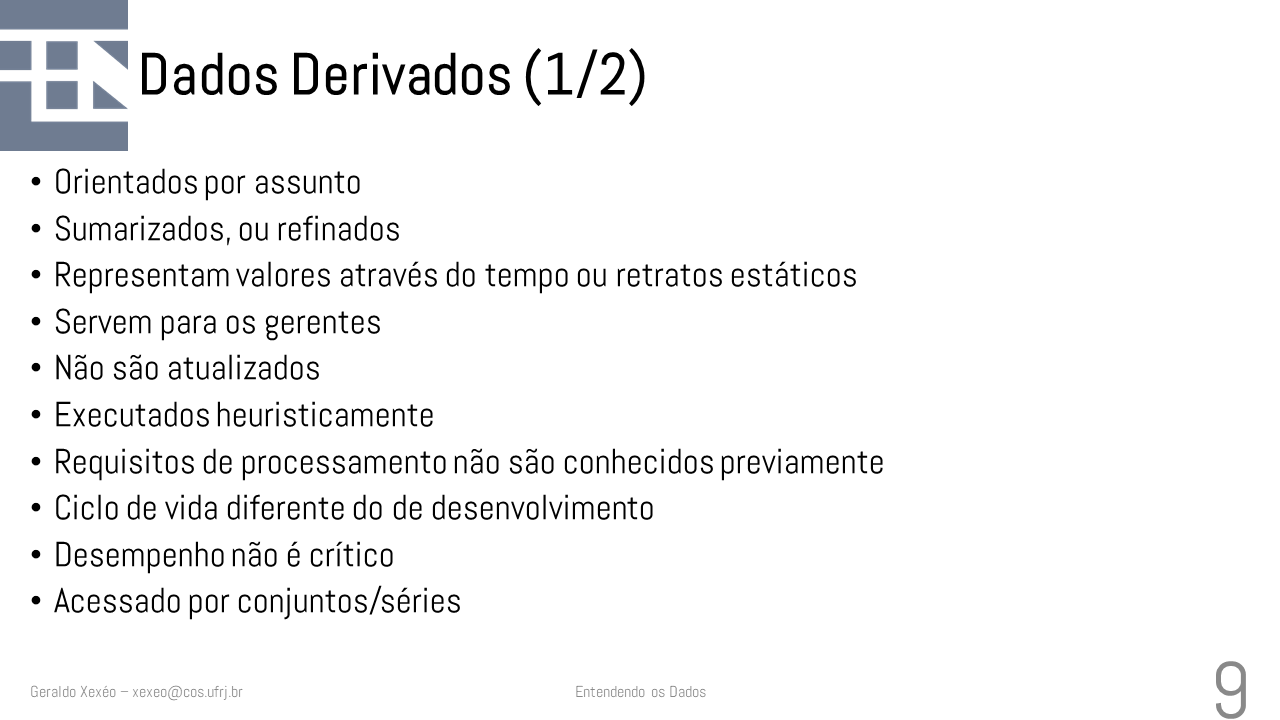
\includegraphics[width=\tam\linewidth,frame]{imagens/dados}
    \caption{Um slide com uma lista de itens. Como a lista é longa, foi dividido em dois.}
    \label{fig:dados}
\end{figure}


A Figura \ref{fig:tres} mostra uma sequência de slides sobre o mesmo tema: riscos de software que se tornaram realidade. Ao invés de colocar vários slides com listas de riscos, optei por usar primeiro uma explicação detalhada passo a passo do acidente do Arianne V, depois uma coleção de notícias recortadas do jornal, que é narrada mais rapidamente, e só no final um slide simples tradicional. Noto que, tanto na notícia do Arianne V quanto nos desastres financeiros, os itens aparecem um a um para a assistência, o que facilita a criação de uma narrativa. Chamo isso de dinâmica do slide, feita na forma de uma animação, e discuto na Seção \ref{sec:din}. O acidente do Arianne V também é mostrado com uma imagem que chama a atenção, servindo para o professor contar a história e chamar atenção dos alunos para a aula.

\begin{figure}
    \centering
    \subfloat{
    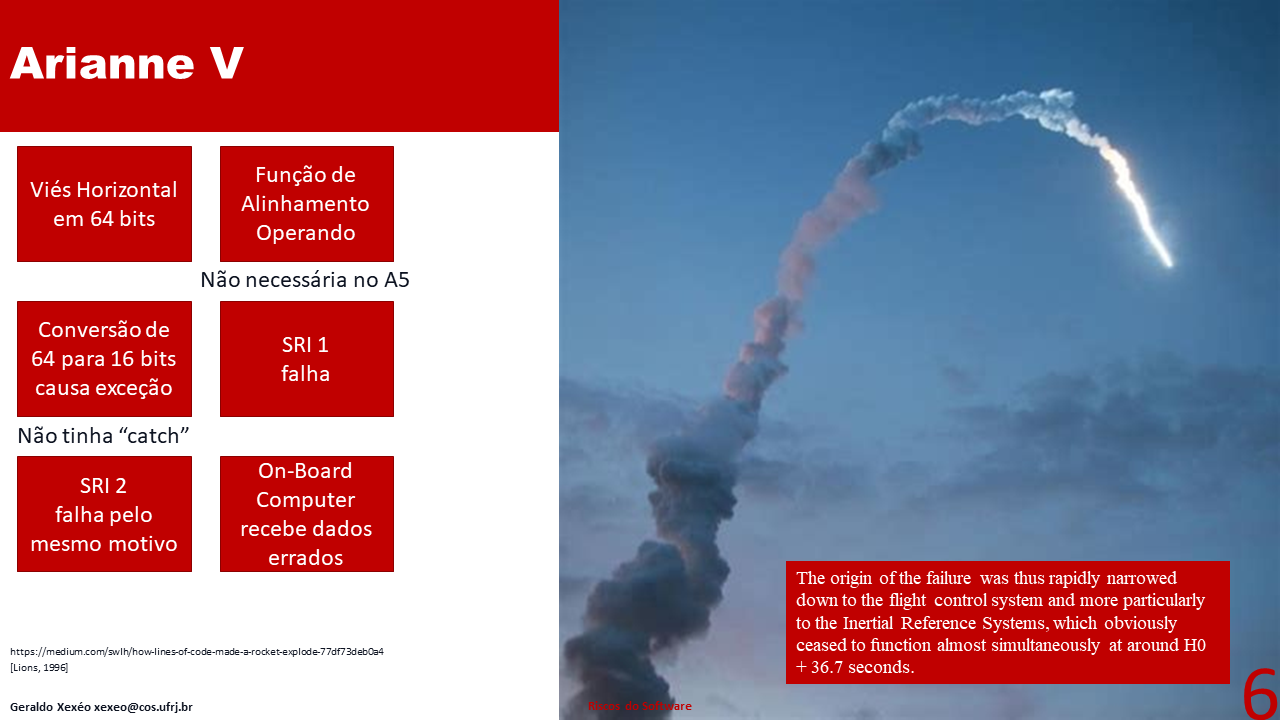
\includegraphics[width=0.3\linewidth,frame]{imagens/arianne.png}
}
   \subfloat{    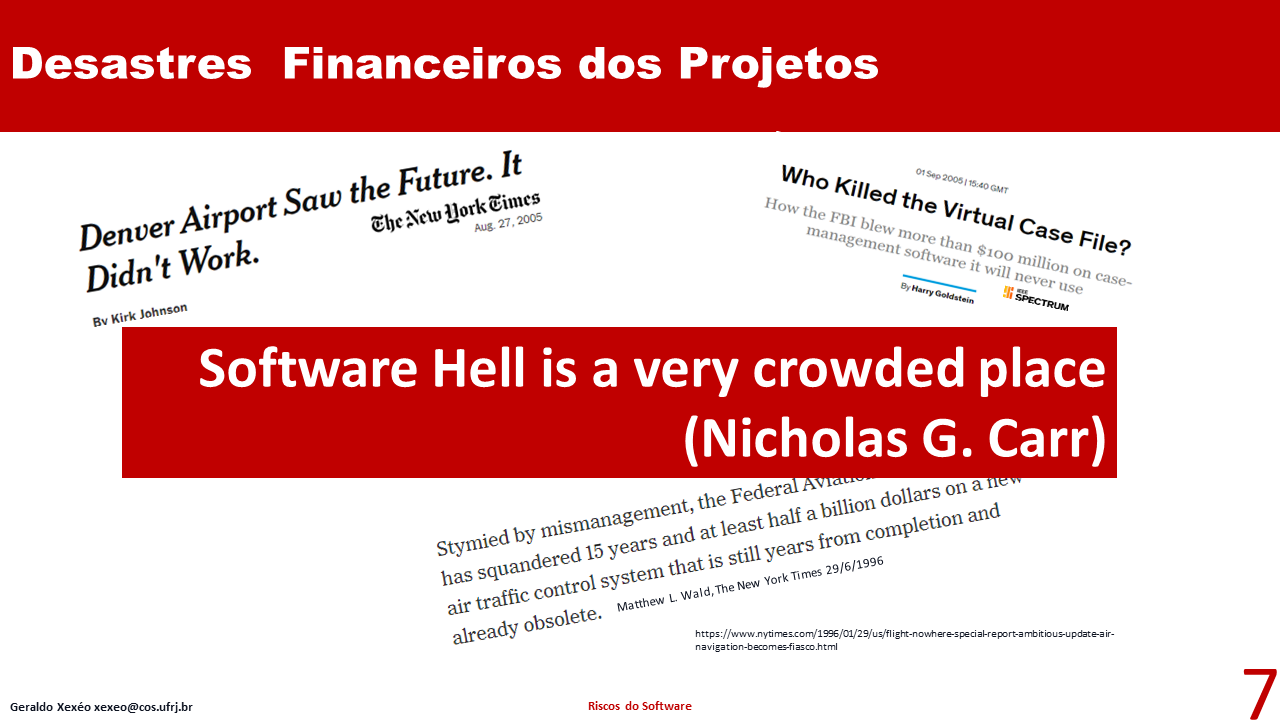
\includegraphics[width=0.3\linewidth,frame]{imagens/hell.png}
    }
\subfloat{
    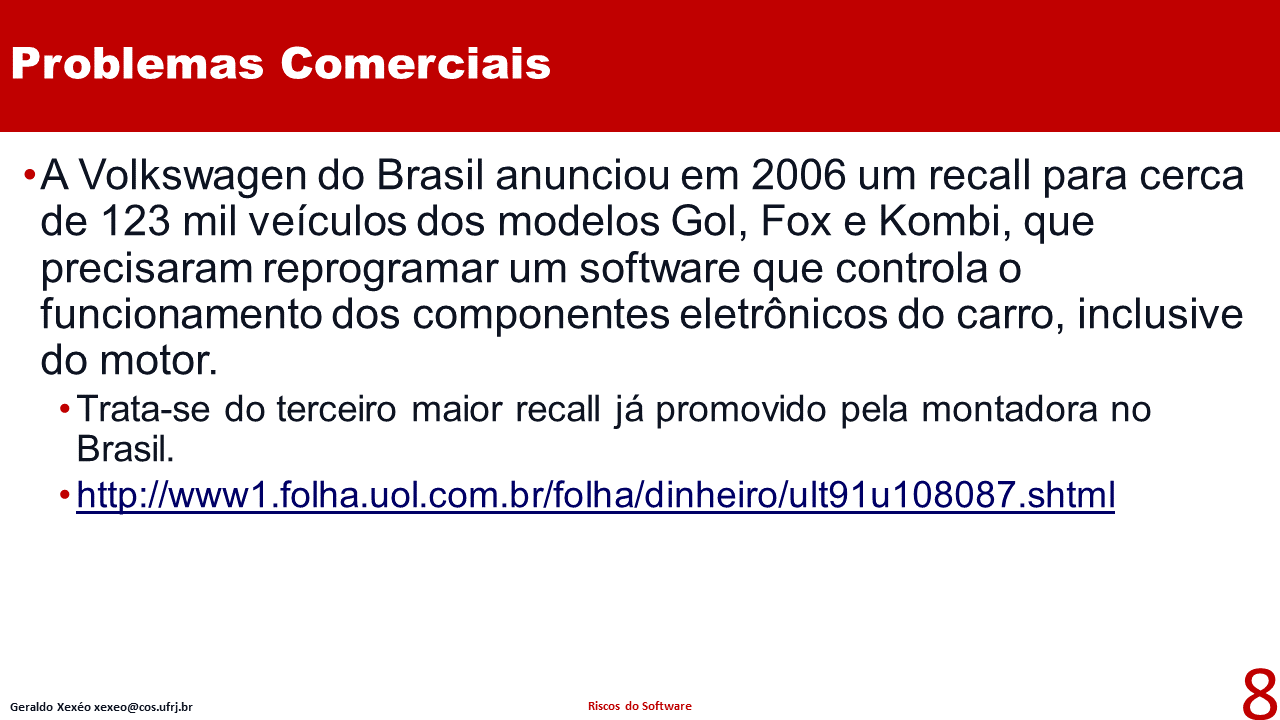
\includegraphics[width=0.3\linewidth,frame]{imagens/problemas.png}
}
\caption{Três slides tratando do mesmo assunto, riscos de software, onde conteúdo e estilo são diferentes. Mesmo assim, eles podem ser percebidos como pertencendo a mesma aula, devido as características comuns do estilo.}
\label{fig:tres}
\end{figure}


É importante que tudo que seja colocado no slide, seja também referenciado de alguma forma, seja pela bibliografia, seja por citações específicas em algum local do slide.
Forneça todas as referências, e \textbf{indique a propriedade intelectual de tudo}. Prefira imagens de domínio público ou com licenças amplas, como \textit{Creative Commons}.


